

\begin{footnotesize}
\begin{verbatim}
create table `shipping_params' as
  select 
    avg   (l_shipdate    - o_orderdate) as ship_mu,
    avg   (l_receiptdate - l_shipdate ) as arrv_mu,
    stddev(l_shipdate    - o_orderdate) as ship_sigma,
    stddev(l_receiptdate - l_shipdate ) as arrv_sigma,
    l_partkey as p_partkey
  from orders,lineitem
  where o_orderkey = l_orderkey
  group by partkey;
alter table params add constraint "p_partkey_pkey" 
  primary key (p_partkey);
-- BEGIN TIMING QUERY --
create temporary table q3_shipping as
  select o_orderkey AS orderkey, o_custkey AS custkey,
    CREATE_VARIABLE(`Normal',row(ship_mu,ship_sigma))
    CREATE_VARIABLE(`Normal',row(arrv_mu,arrv_sigma))
  from  orders,lineitem,shipping_params
  where p_partkey = l_partkey;
   and  o_orderdate = today()
   and  o_orderkey  = l_orderkey;
create temporary table q3_annoyed as
  select custkey from q3_shipping where ship > 120
union all
  select custkey from q3_shipping where arrv > 90;
create temporary table q3_order_increase as
  select o_orderkey, o_custkey,
     CREATE_VARIABLE(`Poisson', row(increase)) *
       l_extended_price * (1.0 - l_discount) as rev
  from (select newc / oldc as increase, custkey 
    from (select o_custkey as custkey, 
             sum(o_orderdate.year-1996.0) AS newc,
             sum(1997.0-o_orderdate.year) AS oldc
      where o_orderdate.year = 1997 
        or  o_orderdate.year = 1996
      group by custkey
     ) as counts
   ) as increase_per_cust,
    orders
  where custkey = o_custkey
 ) as var_increase_per_customer,
 (select lineitem.*,
  from  nation,supplier, lineitem, partsupp
  where n_name = 'japan' and n_nationkey = s_nationkey
   and  s_suppkey = ps_suppkey
   and  ps_partkey = l_partkey
   and  ps_suppkey = l_suppkey
 ) as items_from_japan;
-- BEGIN TIMING SAMPLE --
select avg(confidence),
       expected_sum(rev, q3_annoyed)
from   q3_annoyed,
       (select o_custkey as custkey, rev
        from   q3_revenue_gains
       ) as revenues
where  revenues.custkey = q3_annoyed.custkey;
\end{verbatim}
\end{footnotesize}

\begin{figure}
\begin{center}
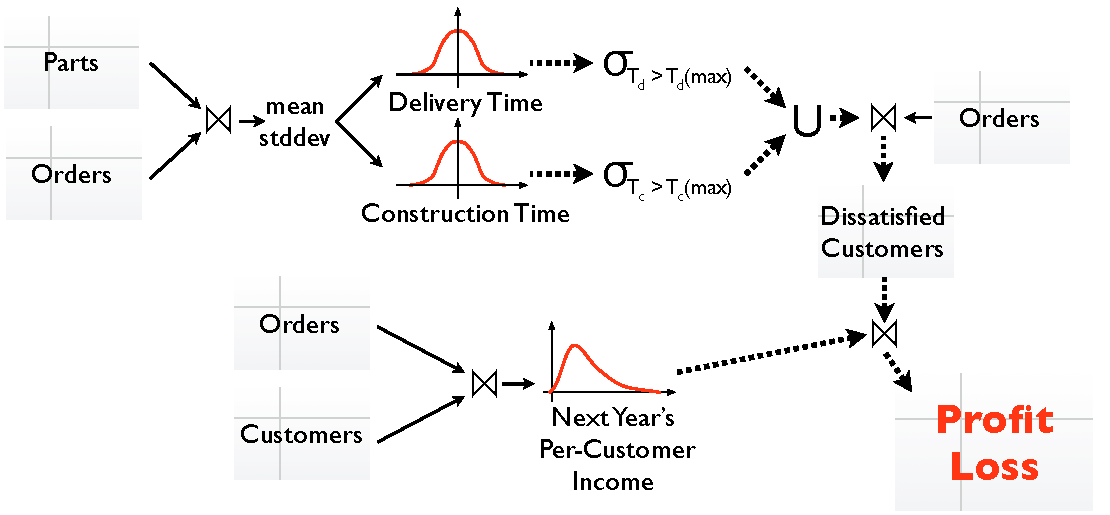
\includegraphics[width=3.1in]{graphics/query3.pdf}
\caption{A dataflow diagram of query 3.  Dotted lines represent probabilistic data.}
\label{fig:query3dataflow}
\end{center}
\end{figure}

Query 3 is based on \cite{MCDB}'s Q1 and Q2 and represented graphically in Figure \ref{fig:query3dataflow}.  A prebuilt table of shipping and construction times is used to parametrize Normal distributions that predict time from order to shipment and time from shipment to arrival.  Note the use of the CREATE\_VARIABLE function to create these variables.  This table is compared against arbitrary customer satisfaction thresholds to generate a probabilistic table containing a customer if the customer was dissatisfied with the shipping times (we selected thresholds that left an average of 10\% of customers dissatisfied by at least one event).  Note that probabilistic variables may be used in WHERE clauses in the same way as deterministic ones.  Separately, the query computes the expected profit for each customer and joins it with the table of dissatisfied customers to estimate the amount of profit lost in the coming year.